\chapter{Video File Formats}


The ISO Base Media File Format is a container for multimedia formats which can contain both audio and video data. It is a general format that represents a basis for a number of other file formats.
As described in the standard ISO/IEC 14496 Part 12 \cite{iso}, it is designed to contain media information for a video in a flexible and extensible format so that the interchange, management, editing, and presentation of a media are facilitated. The information represented includes timing, structure, and media information for a presentation, i.e. one or more motion sequences that can also be combined with audio.

The ISO Base Media File Format has a object-oriented type structure. In fact, files conform to this standard are formed as a sequence of objects, called boxes or sometimes atoms, that contain all the data about the media. Some of these boxes can also contain other boxes. A box consists of a header, followed by the box data. The header contains a unique type identifier, representing the type of the box, and the size of the box. Some boxes may also contain information fields about version number and flags. For these fields, the semantic is the following:

\begin{itemize}
\item \emph{size}: an integer that specifies the number of bytes used by a box, including the fields and all contained boxes.
\item \emph{type}: a four printable characters that identifies the box type.
\item \emph{version}: an integer that specifies the version of the format of the box.
\item \emph{flags}: a set of flags.
\end{itemize}

The sequences of boxes in a file must contain one representation metadata wrapper, i.e. the Movie Box (\emph{moov}). The other boxes that can be found at the first level are File Type Box (\emph{ftyp}), Free Space Boxes (\emph{free}), Movie Fragments (\emph{moof}), Meta-data (\emph{meta}), or Media Data Boxes (\emph{mdat}).

The MP4 File Format, described in the standard ISO/IEC 14496-14 Part 14 \cite{mp4}, and MOV File Format, described in the QuickTime File Format specification \cite{mov}, are derived from the ISO Base Media File Format. In fact, the general structure of the ISO file is fully implemented by both file formats. Each file format introduces new boxes and redefines the values of some fields that are already present in the ISO standard.

In the following, we will give additional information about the structure and the content of the boxes contained in an ISO file.

\section{Box Definitions}

An overall view of an example of a object-oriented structured file of this format can be view in Table \ref{boxtable}. For the complete encapsulation structure, \cite{iso} can be consulted.

\begin{table}[]
\centering
\begin{tabular}{|l|l|l|l|l|l|l|l|l}
\hline
  ftyp &      &      &      &      &      & * & file type and compatibility\\ \hline
  moov &      &      &      &      &      & * & container for all the metadata \\ \hline
       & mvhd &      &      &      &      & * & movie header \\ \hline
       & trak &      &      &      &      & * & container for an individual trak \\ \hline
       &      & tkhd &      &      &      & * & track header\\ \hline
       &      & mdia &      &      &      & * & container for the media information \\ \hline
       &      &      & mdhd &      &      & * & media header \\ \hline
       &      &      & hdlr &      &      & * & handler \\ \hline
       &      &      & minf &      &      & * & media information container \\ \hline
       &      &      &      & vmhd &      &   & video media header \\ \hline
       &      &      &      & smhd &      &   & sound media header \\ \hline
       &      &      &      & hmhd &      &   & hint media header \\ \hline
       &      &      &      & dinf &      & * & data information box \\ \hline
       &      &      &      &      & dref & * & data reference box \\ \hline
       &      &      &      & stbl &      & * & sample table box \\ \hline
       &      &      &      &      & stsd & * & sample descriptions \\ \hline
       &      &      &      &      & stts & * & time-to-sample \\ \hline
       &      &      &      &      & stcs & * & sample-to-chunck \\ \hline
       &      &      &      &      & stcz &   & sample sizes (framing) \\ \hline
       &      &      &      &      & stco & * & chuck offset \\ \hline
       &      &      &      &      & co64 &   & 64-bit chunk offset \\ \hline
       &      &      &      &      & stss &   & sync sample table \\ \hline
       &      &      &      &      & sdtp &   & independent and disposable samples \\ \hline
       &      & udta &      &      &      &   & user-data \\ \hline
       & udta &      &      &      &      &   & user-data \\ \hline
  moof &      &      &      &      &      &   & movie fragment \\ \hline
  mdat &      &      &      &      &      &   & media data container \\ \hline
  free &      &      &      &      &      &   & free space \\ \hline
  meta &      &      &      &      &      &   & metadata \\ \hline
\end{tabular}
\caption{Box types and structure. The boxes with an asterisk (*) are mandatory.}\label{boxtable}
\end{table}

The table shows the boxes that shall occur at the top-level of the file in the left-most column, with indentations representing containments. The boxes that are marked with an asterisk (*) are mandatory. In the following, each box of the table will be described.

\subsection{First Level}

At the first level, we will find:

\subsubsection*{File Type Box (ftyp)}

Since a media file structured accordingly to this file format standard can be compatible with more than one specification, it is not possible to speak of a single type or brand for a file.
The File Type Box (\emph{ftyp}) is a mandatory and unique box that identifies which type represents the best use for a file, along with other compatible specifications. Each brand is described by a four characters code.

The box \emph{ftyp} should be positioned at the top-level of a file before every other box of variable lenghts, such as Movie Box, Free Box, or Media Data Box. Only a box with a fixed-size, such as file signature, may placed before it. The box \emph{ftyp} has three fields:

\begin{itemize}
\item \emph{major\_brand}: identifies the best use specification.
\item \emph{minor\_version}: identifies the version of the major specification.
\item \emph{compatible\_brands}: a list of other compatible specifications.
\end{itemize}

\begin{figure}
  \centering
  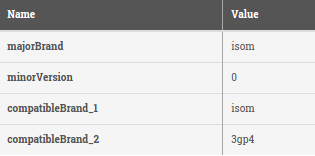
\includegraphics[width=0.5\textwidth]{ftyp}
  \caption{The box \emph{ftyp} of a file container of a video acquired with a Samsung Galaxy S3.}\label{fig:ftyp}
\end{figure}

An example can be seen in Fig. \ref{fig:ftyp} showing the box \emph{ftyp} of a video acquired with a Samsung Galaxy S3.

\subsubsection*{Movie Box (moov)}

The Movie Box (\emph{moov}) is a mandatory and unique box that contains the necessary metadata for a presentation and is placed at the top-level of a file. Although it is not explicitly required, it is normally located close to the beginning or end of a file. It is also a container for other boxes.

\subsubsection*{Movie Fragment Box (moof)}

The Movie Fragment Box (\emph{moof}) is an optional box that extends the media in time, providing additional information that would previously have been present in the Movie Box. It is placed at the top-level of a file and contains a Movie Fragment Header Box (\emph{mfhd}) and one or more Track Fragment Boxes (\emph{traf}). The Movie Fragment Boxes must be placed in the file accordingly to their sequence number.

\subsubsection*{Media Data Box (mdat)}

The Media Data Box (\emph{mdat}) contains the media data. Since a presentation can contain zero or more Media Data boxes, it is a optional box. It has a field that specifies the size of the contained media data.

\subsubsection*{Free Space Box (free)}

The Free Space Box (\emph{free}) is an optional box that can be placed at the top-level of a file or can be contained in other boxes. Usually, the content of this box can be ignored and therefore deleted, without affecting the presentation.

\subsubsection*{Meta Box (meta)}

The Meta Box (\emph{meta}) is an optional box that contains annotative metadata. This box may be located at the top-level of the file, or inside the Movie Box (\emph{moov}) or the Track Box (\emph{trak}). If present, it is required to contain a Handler Reference Box (\emph{hdlr}) that indicates the format of the content of the Meta Box.

\subsection{Second Level}

At the second level, we will find:

\subsubsection*{Movie Header Box (mvhd)}

The Movie Header Box (\emph{mvhd}) is a mandatory and unique box that is located inside the Movie Box. It is used to specify characteristics of an entire video. The fields contained in the box \emph{mvhd} are the following:

\begin{itemize}
\item \emph{version}: an integer that specifies the number of bytes for this Movie Header Box.
\item \emph{creation\_time}: an integer that represents the creation time of a video.
\item \emph{modification\_time}: an integer that represents the most recent time the video was modified.
\item \emph{timescale}: an integer that specifies the time-scale for the entire media. It indicates how many units pass in one second.
\item \emph{duration}: an integer representing the length, in terms of time, of the video.
\item \emph{rate}: it indicates the preferred rate to play the video.
\item \emph{volume}: it indicates the preferred audio volume to play the video.
\item \emph{matrix}: it represents a geometrical transformation matrix for the video.
\item \emph{next\_track\_ID}: a non-zero integer that specifies an ID value to use for the next track to be added to the video.
\end{itemize}

It is advised that the Movie Header Box should be placed first in its container.

\begin{figure}
  \centering
  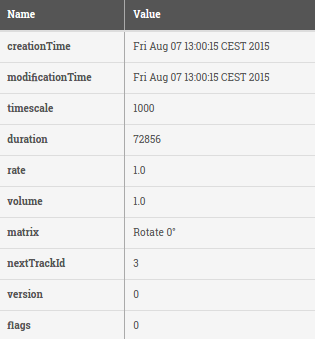
\includegraphics[width=0.5\textwidth]{mvhd}
  \caption{The box \emph{mvhd} of a file container of a video acquired with a Samsung Galaxy S3.}\label{fig:mvhd}
\end{figure}

An example can be seen in Fig. \ref{fig:mvhd} showing the box \emph{mvhd} of a video acquired with a Samsung Galaxy S3.

\subsubsection*{Track Box (trak)}

The Trak Box (\emph{trak}) is a mandatory box for a file that is located inside the Movie Box. A video contained one or more tracks, such as audio or video tracks, with each track independent from the others. Tracks can either be media tracks, containing media data, or hint tracks, containing information for streaming protocol. Every presentation must have at least one media track within an ISO file.

\subsubsection*{User Data Box (udta)}

The User Data Box (\emph{udta}) is an optional box that can either be contained inside a Movie Box or a Track Box. It contains objects that specify user information about the presentation or the track. It contains a set of boxes with more box types that indicate more precisely their content.

It is advised that the User Data Box should be placed last in its container.

\subsection{Third Level}

At the third level, we will find:

\subsubsection*{Track Header Box (tkhd)}

The Track Header Box (\emph{tkhd}) is a mandatory and unique box that specifies the characteristics of a track. It is contained inside the Track Box. It contains the following fields:

\begin{itemize}
\item \emph{version}: an integer that specifies the version of the box. Can either be 0 or 1.
\item \emph{flags}: an 24-bit integer whose values indicates a track that is enabled (\emph{Track\_enabled}), a track that must be used for in the video (\emph{Track\_in\_movie}), or a track that must be used in the preview of the video.
\item \emph{creation\_time}: an integer that indicates the creation time of a video.
\item \emph{modification\_time}: an integer that represents the most recent time the video was modified.
\item \emph{track\_ID}: an integer number that uniquely identifies a track.
\item \emph{duration}: an integer that indicates the length, in terms of time, of the video.
\item \emph{layer}: it specifies the order \emph{front-to-back} of the video tracks.
\item \emph{alternate\_group}: an integer that specifies a group of tracks. It can either be 0, meaning that no relations between tracks are present, or 1, meaning that there are relations between tracks of different groups.
\item \emph{volume}: it specifies the relative audio volume of the track.
\item \emph{matrix}: it represents a transformation matrix for the video.
\item \emph{width} and \emph{height}: they specify the resolution of the video track.
\end{itemize}

It is advised that the Header Header Box should be placed first in its container.

\begin{figure}
  \centering
  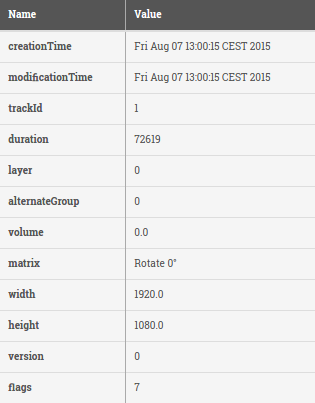
\includegraphics[width=0.5\textwidth]{tkhd-video}
  \caption{The box \emph{tkhd} of a file container of a video acquired with a Samsung Galaxy S3. This box represents an header for a video track.}\label{fig:tkhd-video}
\end{figure}

Examples can be seen in Fig. \ref{fig:tkhd-video} and Fig. \ref{fig:tkhd-audio}, showing the box \emph{tkhd} of a video acquired with a Samsung Galaxy S3, both for video and audio tracks.

\begin{figure}
  \centering
  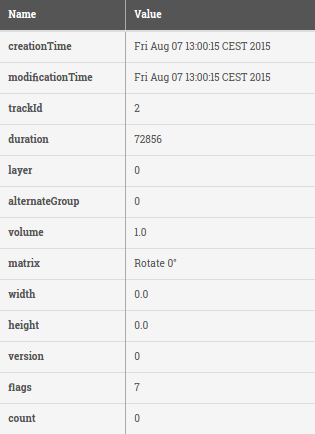
\includegraphics[width=0.5\textwidth]{tkhd-audio}
  \caption{The box \emph{tkhd} of a file container of a video acquired with a Samsung Galaxy S3. This box represents an header for an audio track.}\label{fig:tkhd-audio}
\end{figure}


\subsubsection*{Media Box (mdia)}

The Media Box (\emph{mdia}) is mandatory and unique box within the file and it is contained inside the Track Box. It contains all the objects that specify information about the media data in a track.

\subsection{Forth Level}

At the forth level, we will find:

\subsubsection*{Media Header Box (mdhd}

The Media Header Box (\emph{mdhd}) is a mandatory and unique box contained inside a Media Box. It declares all the information relevant to the media in a track. The box \emph{mdhd} contains the following fields:

\begin{itemize}
\item \emph{version}: an integer that indicates the version of this box.
\item \emph{creation\_time}: an integer that indicates the creation time of the media track.
\item \emph{modification\_time}: an integer that indicates the most recent time the media track was modified.
\item \emph{timescale}: an integer that specifies the time-scale for the entire media. It indicates how many units pass in one second.
\item \emph{duration}: an integer representing the length, in terms of time, of the media track.
\item \emph{language}: it specifies the language code for the media track.
\end{itemize}

It is advised that the Media Header Box should be placed first in its container.

\subsubsection*{Handler Reference Box (hdlr)}

The Handler Reference Box (\emph{hdlr}) is a mandatory and unique box that is contained inside a Media Box or a Meta Box. When inside a Media Box, it specifies the nature of the media track. For example, a video track will be handled by a video handler and a sound track will be handled by a sound handler. When inside a Meta Box, it indicates the format of content of the Meta box.

It contains the following fields:

\begin{itemize}
\item \emph{version}: an integer that specifies the version of the box.
\item \emph{handler\_type}: when inside a Media Box, it is an integer containing 'vide' for video tracks, 'soun' for sound track or 'hint' for hint track; when inside a Meta Box,  it contains a value indicating the format of the content of the Meta Box.
\item \emph{name}: a string of characters that associates a human-readable name for the media track type.
\end{itemize} 

While \emph{handler\_type} value is consistent, \emph{name} can change along different devices. For example, for a Samsung Galaxy S3 the handler for video tracks is called 'VideoHandle' and the handler for audio tracks is called 'SoundHandle', while for a Apple iPhone 5 they are called 'Core Media Video' and 'Core Media Audio' respectively.

\subsubsection*{Media Information Box (minf)}

The Media Information Box (\emph{minf}) is a mandatory and unique box that is located inside the Media Box. It contains characteristic information about the media track.

\subsection{Fifth Level}

At the fifth level, we will find:

\subsubsection*{Video Media Header Box (vmhd)}

The Video Media Header Box (\emph{vmhd}) is media information header box located inside the Media Information Box. It contains general information about the video track. The box \emph{vmhd} has the following fields:

\begin{itemize}
\item \emph{version}: an integer that specifies the version of the box.
\item \emph{graphicmode}: it specifies a composition mode for the video track.
\item \emph{opcolor}: is an RGB value that is available for use by the graphics modes.
\end{itemize}

\subsubsection*{Sound Media Header Box (smhd)}

The Sound Media Header Box (\emph{smhd}) is a media information header box located inside the Media Information Box. It contains general information about the audio track. The box \emph{smhd} has the following fields:

\begin{itemize}
\item \emph{version}: an integer that specifies the version of the box.
\item \emph{balance}: a number that places mono audio tracks in a stereo space.
\end{itemize}

\subsubsection*{Hint Media Header Box (hmhd)}

The Hint Media Header Box (\emph{hmhd}) is a media information header box located inside the Media Information Box. It contains general information about the hint track.

\subsubsection*{Data Information Box (dinf)}

The Data Information Box (\emph{dinf}) is a unique box that is mandatory within a Media Information Box. It can also be located inside a Meta Box and contains the location of the media information in a track.

\subsubsection*{Sample Table Box (stbl)}

The Sample Table Box (\emph{stbl}) is a mandatory and unique box situated inside the Media Information Box. It contains entries tables that specify the location of the sample, the type of the sample, determine their size and offset within the container. Such tables are contained in sub-boxes that indicate information about sample description (\emph{stsd}), sample size (\emph{stcz}), sample to chunk (\emph{stcs}), chunck offset (\emph{stco}), etc.

\subsection{Sixth Level}

At the sixth level, we will find:

\subsubsection*{Data Reference Box (dref)}

The Data Reference Box (\emph{dref}) is a mandatory and unique box located within a Data Information Box. It contains a table of data references (URLs) that specifies the location of the media data used within the video file.